\chapter{Теоретическая часть}
\section{Полупроводник}
Рассматривая полупродники, мы будем говорить о кристалических телах. Для анализа таких тел необходимо решить уравнение Шредингера для нахождения, к примеру, энергитеских уровней. В целях упрощения задачи и сохранения наиболее характерных черт системы в Зонной теории вводится ряд допущений: 
\begin{enumerate}
	\item Атомные ядра являются неподвижными источниками поля, действующего на электроны;
	\item Расположения атомных ядер в пространстве является строго переодичным: они распологаются в узлах идеальной кристалической решетки;
	\item Взаимодейсвие электронов друг с другом заменяется некоторым внешним полем.
\end{enumerate}

\subsection{Зонная структура}
В следствии симметрии и переодичности идеального кристалла по разлиным направлениям и теории Блоха, для описания дисперсии электронов используют зоны Бриллюэна \cite{Kalashnikov}. Так как закон дисперсии переодичен на всем кристалле, для его описания можно использовать только первую зону Бриллюэна. 

\begin{figure}[h]
	\centering
    \begin{minipage}[b]{0.4\textwidth}
	    \includegraphics[width=\textwidth]{assets/Brullien}
	    \caption{Зонная структура $GaAs$}
	\end{minipage}
	\hfill
	\begin{minipage}[b]{0.4\textwidth}
		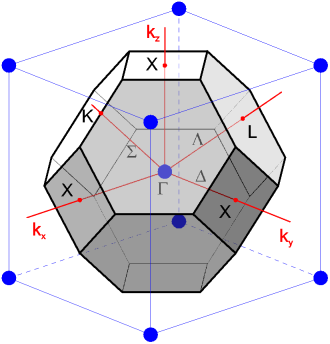
\includegraphics[width=\textwidth]{assets/ZnLaer}
	    \caption{Элементарная ячейка типа Цинковой обманки}
	\end{minipage}
\end{figure}

Для наглядного представления и сравнения полупроводников и других материалов удобно использовать зонную диаграмму. 


\subsection{Плотсноть состояний}
\subsection{Концентрация носителей заряда}
\subsubsection{Собственный полупроводник}
\subsubsection{Легированный полупроводник}
